11. \begin{figure}[ht!]
\center{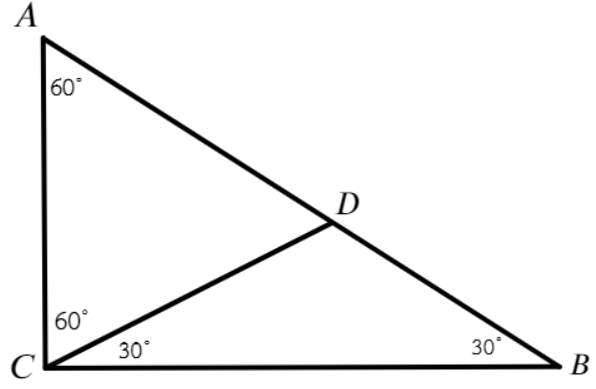
\includegraphics[scale=0.35]{g11.png}}
\end{figure}\\
Треугольник $ACD$ равносторонний, значит все его углы равны $60^\circ.$ Тогда $\angle DCB=\angle C-\angle ACD=90^\circ-60^\circ=30^\circ,\ \angle DBC=180^\circ-\angle A-\angle C=180^\circ-60^\circ-90^\circ=30^\circ.$ Поэтому в треугольнике $BCD$ равны углы при основании $BC$ и он является равнобедренным, ч.т.д.\\
